\documentclass{article}
\usepackage[utf8]{inputenc}

\usepackage[utf8]{inputenc}
\usepackage[spanish,es-tabla,es-nodecimaldot]{babel}
\usepackage{amsmath,amsthm,amsfonts,amssymb,mathtools,dsfont,mathrsfs}
\usepackage{enumerate,graphicx,xcolor}
\usepackage{lmodern}
\usepackage[T1]{fontenc}
\usepackage[left=2cm,top=2.5cm,right=2cm,bottom=2.5cm]{geometry}
\usepackage[activate={true,nocompatibility},final,tracking=true,kerning=true,spacing=true,factor=1100,stretch=10,shrink=10]{microtype}
\usepackage{hyperref}


%\DeclarePairedDelimiter{\norm}{\lVert}{\rVert}




\newcommand{\N}{\mathbb{N}}
\newcommand{\R}{\mathbb R}
\newcommand{\Z}{\mathbb Z}
\newcommand{\Rbar}{\overline{\mathbb R}}
\newcommand{\F}{\mathscr F}
\newcommand{\A}{\mathscr A}
\newcommand{\To}{\Rightarrow}
\newcommand{\C}{\mathscr C}
\newcommand{\La}{\mathscr L_A}
\newcommand{\B}{\mathcal B}
\newcommand{\Q}{\mathbb Q}
\renewcommand{\epsilon}{\varepsilon}
\renewcommand{\L}{\mathcal L}
\renewcommand{\d}{\mathrm d}
\newcommand{\abs}[1]{\left| #1 \right|}
\newcommand{\pts}[1]{\left( #1 \right)}
\newcommand{\norm}[1]{\left\lVert#1\right\rVert}
\renewcommand{\P}[1]{\mathbb P\left( #1 \right)}
\newcommand{\E}[1]{\mathbb E \left( #1 \right)}


\newcommand{\ols}[1]{\mskip.5\thinmuskip\overline{\mskip-.5\thinmuskip {#1} \mskip-.5\thinmuskip}\mskip.5\thinmuskip} % overline short
\newcommand{\olsi}[1]{\,\overline{\!{#1}}} % overline short italic
\makeatletter
\newcommand\closure[1]{
  \tctestifnum{\count@stringtoks{#1}>1} %checks if number of chars in arg > 1 (including '\')
  {\ols{#1}} %if arg is longer than just one char, e.g. \mathbb{Q}, \mathbb{F},...
  {\olsi{#1}} %if arg is just one char, e.g. K, L,...
}
% FROM TOKCYCLE:
\long\def\count@stringtoks#1{\tc@earg\count@toks{\string#1}}
\long\def\count@toks#1{\the\numexpr-1\count@@toks#1.\tc@endcnt}
\long\def\count@@toks#1#2\tc@endcnt{+1\tc@ifempty{#2}{\relax}{\count@@toks#2\tc@endcnt}}
\def\tc@ifempty#1{\tc@testxifx{\expandafter\relax\detokenize{#1}\relax}}
\long\def\tc@earg#1#2{\expandafter#1\expandafter{#2}}
\long\def\tctestifnum#1{\tctestifcon{\ifnum#1\relax}}
\long\def\tctestifcon#1{#1\expandafter\tc@exfirst\else\expandafter\tc@exsecond\fi}
\long\def\tc@testxifx{\tc@earg\tctestifx}
\long\def\tctestifx#1{\tctestifcon{\ifx#1}}
\long\def\tc@exfirst#1#2{#1}
\long\def\tc@exsecond#1#2{#2}
\makeatother

\newtheorem{lemma}{Lema}
\newtheorem{theorem}{Teorema}

\setlength\parindent{0pt}
\setlength\parskip{4pt}


\title{Cómputo científico para probabilidad y estadística. Tarea 5.\\
Simulación Estocástica, introducción.}
\author{Juan Esaul González Rangel}
\date{Octubre 2023}



\begin{document}

\maketitle


\begin{enumerate}

    \item Definir la cdf inversa generalizada $F^-_X$ y demostrar que en el caso de 
    variables aleatorias continuas esta coincide con la inversa usual. Demostrar 
    además que en general para simular de $X$ podemos simular $u \sim U (0, 1)$ y 
    $F^-_X (u)$ se distribuye como $X$. [1 punto]

    \begin{proof}
        Sea $F$ una función de distribución. La inversa generalizada $F^-$ está definida como,

        \[ F^-(x) = \inf\{ y : F(y) \ge x \}.\]

        Si $F$ es la función de distribución de una variable aleatoria continua (cuya densidad
        es continua), entonces $F$ es monótona creciente, y por lo tanto es invertible. 
        Como $F$ es monótona creciente, también lo es $F^{-1}$, de donde se tiene

        \[ F^-(x) = \inf\{ y : F(y) \ge x \} = \inf\{ y : y \ge F^{-1}(x) \} = F^{-1}(x). \]

        Lo anterior se cumple para todo $x \in \R$, es decir $F^-(x)=F^{-1}(x), \forall x \in \R$.

        Mostramos ahora que si $u\sim U(0,1)$ entonces $F_X^-$ se distribuye como $X$. Primero 
        notemos que por definición de $F^-$ se satisface que 

        \[ F_X(F_X^-(x)) \ge x. \]

        También tenemos que $x \in \{ y : F_X(y) \ge F_X(x) \}$ por lo que

        \[ F^-_X(F_X(x)) = \inf \{ y : F_X(y) \ge F_X(x) \} \le x. \]

        Mostraremos la igualdad de los conjuntos $\{(y,x) : F_X^-(y) \le x\} = \{ (y,x) : F_X(x) \ge y\}$.
        Primero sean $y,x$ tales que $F_X^-(y) \le x$, por las propiedades anteriores,

        \begin{align*}
            y &\le F_X( F_X^-(x) ) \le F_X(x).
        \end{align*}

        Sean ahora $x,y$ tales que $y \le F_X(x)$, entonces

        \begin{align*}
            x \ge F^-_X( F_X(x) ) \ge F_X^-(y).
        \end{align*}

        De las dos implicaciones anteriores tenemos que $\{(y,x) : F_X^-(y) \le x\} = \{ (y,x) : F_X(x) \ge y\}$.
        Sea $u\sim U(0,1)$

        \begin{align*}
            \P{ F_X^-(U) \le x } = \P{U \le F_X(x)} = F_X(x).
        \end{align*}

        Lo anterior se cumple para todo $x \in \R$. Como la función de distribución caracteriza
        la distribución, concluimos que $X \overset d{=} F_X^-(U)$.

    \end{proof}

    \item Implementar el siguiente algoritmo para simular variables aleatorias 
    uniformes:
    
    \[ x_i = 107374182x_{i-1} + 104420x_{i-5} \mod 2^{31} - 1\]
    
    regresa $x_i$ y recorrer el estado, esto es $x_{j-1} = x_j ; j = 1, 2, 3, 4, 5;$ 
    ¿parecen $U (0, 1)$? [1 punto]

    En el archivo \texttt{Tarea5.py} la función tiene el nombre \texttt{simulate\_unif}. Esta
    función toma dos parámetros, el primero es la cantidad de variables a simular y el segundo
    que es opcional es la semilla a usar. En este caso la semilla es una lista con 5 números y su
    valor predeterminado es \texttt{[57,189,42,26,4]}.

    El siguiente ejemplo corto muestra el uso del algoritmo,

    \begin{lstlisting}[language=Python]
simulate_unif(20)\end{lstlisting}

    La salida es una lista con 20 simulaciones uniformes en $(0,1)$. Notemos que no hace
    falta especificar la semilla porque hay valores preasignados, pero si lo preferimos 
    es posible hacerlo.

\begin{lstlisting}[language=Python]
array([[0.20277159],
    [0.33821995],
    [0.33366523],
    [0.5844814 ],
    [0.14562601],
    [0.15818634],
    [0.02168181],
    [0.61616571],
    [0.48205825],
    [0.89928987],
    [0.50309849],
    [0.98820393],
    [0.67741769],
    [0.08572004],
    [0.16774989],
    [0.03575408],
    [0.69187728],
    [0.06325333],
    [0.91457816],
    [0.47367591]])\end{lstlisting}

    Para verificar si los valores simulados son próximos a muestras uniformes en $(0,1)$
    podemos usar varios métodos, pero es necesario obtener una muestra más grande.

    Al realizar 10,000 simulaciones con nuestro algoritmo, encontramos que la media es 0.5010,
    la varianza es 0.082790 y los límites superior e inferior son 0.00006 y 0.99995. En todos 
    los casos, estos están próximos a lo que se esperaría encontrar de una muestra de variables
    aleatorias uniformes en $(0,1)$. 

    Podemos apreciar mejor el comportamiento de la muestra al usar un histograma de frecuencia
    relativa.

    \begin{center}
        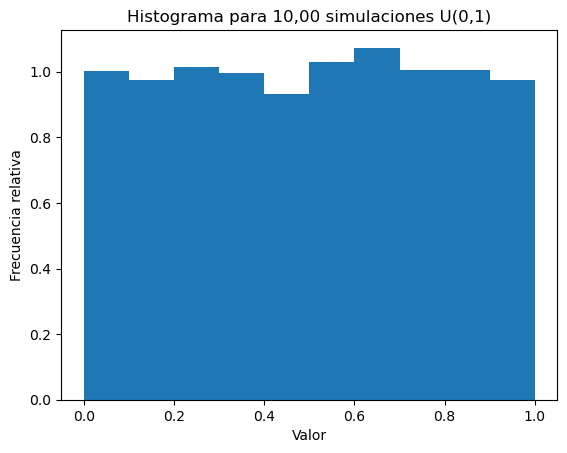
\includegraphics[width=0.6\textwidth]{hist_unif.png}
    \end{center}

    Como podemos notar, el histograma de las simulaciones es muy parecido a una densidad uniforme
    en $(0,1)$. 
    
    Una manera más precisa de evaluar la proximidad de la distribución empírica
    de los valores simulados a la distribución objetivo es mediante el uso de una prueba de bondad 
    de ajuste. Al aplicar la prueba de Kolmogorov-Smirnov para evaluar si la muestra proviene de
    una distribución uniforme en $(0,1)$ encontramos un p-valor de 0.4329928620961334, es decir,
    no hay evidencia suficiente para rechazar que la prueba provenga de esta distribución.

    Con lo anterior, evaluamos que para propósitos sencillos, la muestra que obtuvimos se comporta
    como una muestra de v. a. i. i. d. uniformes en $(0,1)$. Sin embargo, existen pruebas más sofisticadas
    que se aplican a diversos algoritmos con el propósito de verificar con cuál de ellos se pueden
    encontrar simulaciones que mejor aproximen muestras aleatorias. Se podría dar el caso de que al
    usar una prueba más compleja, la muestra ya no presente el comportamiento característico de 
    la distribución uniforme.


    \item ¿Cuál es el algoritmo que usa \texttt{scipy.stats.uniform} para generar 
    números aleatorios? ¿Cómo se pone la semilla? ¿y en \texttt{R}? [1 punto]

    % Kolmogorov-Smirnov, correlación, Lehmann, Die Hard
    % https://justinbois.github.io/bootcamp/2020/lessons/l23_random_number_generation.html

    De acuerdo con la documentación de Scipy, la generación de números aleatorios se realiza llamando
    a las funciones \texttt{Random State} o \texttt{Random Generator} de Numpy. En la documentación
    de Numpy se menciona que hasta la versión 1.17.3, el algoritmo por defecto para la generación
    de números aleatorios era el algoritmo de Mersenne Twister, pero a partir de la versión 1.17.4
    se cuenta con el algoritmo PCG64 que ofrece varias ventajas, entre ellas un mejor desempeño 
    estadístico.

    En cuanto a la semilla, hay dos formas principales de agregarla en Scipy, la primera es agregarla
    directamente dentro del parámetro \texttt{random\_state} de una función \texttt{rvs}, la segunda forma
    es modificar directamente la semilla de Numpy, ya que Scipy llama a Numpy para crear las simulaciones.
    En Numpy hay dos maneras de cambiar la semilla, la primera es a través de la instrucción \texttt{numpy.random.seed()}
    que modifica la semilla global para cada vez que se llame a \texttt{numpy.random}, la segunda forma
    es instanciando un generador de números pseudoaleatorios y modificando directamente la semilla
    en él, lo que se logra mediante \texttt{rg = np.random.default\_rng(seed=semilla)}. La diferencia es que
    cuando se trabaja con una instancia del generador, la modificación de la semilla únicamente afecta
    a las simulaciones que se realicen desde este generador (con \texttt{rg.uniform(size=10)}, por ejemplo).

    En \texttt{R}, el algoritmo predeterminado es también Mersenne Twister, aunque en la documentación
    se puede encontrar una lista de otros algoritmos que se pueden usar, entre ellos están
    Super-Duper, Wichmann-Hill, Marsaglia-Multicarry, Knuth-TAOCP-2002, Knuth-TAOCP y L'Ecuyer-CMRG.

    Es posible modificar con qué algoritmo se trabaja en \texttt{R} cuando se ejecuta la instrucción usual \texttt{runif()}.
    Para modificar la semilla en \texttt R se utiliza el comando \texttt{set.seed()}.

    \textbf{Referencias de la documentación:}

    \url{https://justinbois.github.io/bootcamp/2020/lessons/l23_random_number_generation.html}

    \url{https://github.com/numpy/numpy/blob/7ccf0e08917d27bc0eba34013c1822b00a66ca6d/numpy/random/mtrand/mtrand.pyx}

    \url{https://consultglp.com/wp-content/uploads/2016/12/r-techniques-in-generating-random-numbers.pdf}

    \url{https://numpy.org/devdocs/reference/random/generator.html}

    \url{https://numpy.org/devdocs/reference/random/bit_generators/pcg64.html#numpy.random.PCG64}


    \item ¿En \texttt{scipy} que funciones hay para simular una variable aleatoria 
    genérica discreta? ¿tienen preproceso? [1 punto]

%     rk_double(rk_state *state)
% {
    %  /* shifts : 67108864 = 0x4000000, 9007199254740992 = 0x20000000000000 */
%     long a = rk_random(state) >> 5, b = rk_random(state) >> 6;
%     return (a * 67108864.0 + b) / 9007199254740992.0;
% }
% https://github.com/numpy/numpy/blob/7ccf0e08917d27bc0eba34013c1822b00a66ca6d/numpy/random/mtrand/mtrand.pyx#L3671

    Existe una amplia lista de variables aleatorias discretas que pueden ser simuladas con Scipy. Concretamente
    en su página se mencionan 

    \begin{quote}
    Bernoulli Distribution,
    Beta-Binomial Distribution,
    Binomial Distribution,
    Boltzmann (truncated Planck) Distribution,
    Planck (discrete exponential) Distribution,
    Poisson Distribution,
    Geometric Distribution,
    Negative Binomial Distribution,
    Hypergeometric Distribution,
    Fisher’s Noncentral Hypergeometric Distribution,
    Wallenius’ Noncentral Hypergeometric Distribution,
    Negative Hypergeometric Distribution,
    Zipf (Zeta) Distribution,
    Zipfian Distribution,
    Logarithmic (Log-Series, Series) Distribution,
    Discrete Uniform (randint) Distribution,
    Discrete Laplacian Distribution,
    Yule-Simon Distribution.
    \end{quote}

    Todas estas distrbuciones son instancias específicas de la clase más general \texttt{rv\_discrete}
    que permite definir para cualquier conjunto de valores y sus probabilidades asociadas, un generador de números
    aleatorios con esa distribución. La ventaja de que Scipy sea orientado a objetos es que al crear unan
    ueva instancia de la clase \texttt{rv\_discrete}, esta hereda todos los atributos de la clase madre, y
    por lo tanto al especificar una nueva distribución discreta, ya se cuenta con todas las herramientas
    usuales de las distribuciones que vienen implementadas en Scipy, como pmf, rvs, cdf, etcétera.

    Otra manera de simular variables aleatorias discretas genéricas es mediante la función de Numpy \texttt{numpy.random.choice}.
    Como su nombre lo indica, esta función permite especificar un vector de valores posibles y sus probabilidades.
    La principal diferencia es que esta función no genera un objeto, por lo que únicamente sirve para
    simulaciones puntuales y no para realizar más operaciones con la distribución.

    En cuanto al preproceso, las implementaciones de las variables aleatorias comunes (Bernoulli, Poisson,
    Geométrica, etcétera) sustituyen la implementación genérica de \texttt{rvs} por una versión ad hoc, lo 
    que posiblmente resulta en mayor eficacia y menor tiempo de ejecución. En el caso de las variables
    que toman una cantidad infinita de valores (como Poisson), el preproceso o método ad hoc también
    permite hacer esto que no sería posible usando únicamente la lista de valores y probabilidades.

    \textbf{Referencias de la documentación:}
    
    \url{https://github.com/scipy/scipy/blob/v1.11.3/scipy/stats/_discrete_distns.py#L111-L173}

    \url{https://numpy.org/doc/stable/reference/random/generated/numpy.random.choice.html}

    \url{https://docs.scipy.org/doc/scipy/tutorial/stats/discrete.html#discrete-distributions-in-scipy-stats}

    

    \item Implementar el algoritmo Adaptive Rejection Sampling y simular de una 
    Gama(2, 1) 10,000 muestras. ¿cuando es conveniente dejar de adaptar la envolvente?
     (vea alg. A.7, p. 54 Robert y Casella, 2da ed.) [6 puntos]

    Para la implementación completa del algoritmo se crearon varias funciones en el archivo \texttt{Tarea 5.py},
    A continuación una descripción sencilla de cada una,

    \begin{itemize}
        \item \texttt{log\_gamma\_dens(point,alpha=2,beta=1)}: Esta función calcula el logaritmo 
        de una densidad gamma con parámetros dados (por defecto 2 y 1) evaluada en un punto $x$.
        \item \texttt{gamma\_dens(point,alpha=2,beta=1)}: Esta función calcula una densidad gamma 
        con parámetros dados (por defecto 2 y 1) evaluada en un punto $x$.
        \item \texttt{create\_line(start,end,point\_to\_evaluate)}: Eta función encuentra la ecuación 
        de una recta que pase por los puntos \texttt{start} y \texttt{end} y la evalúa en un punto
        especificado.
        \item \texttt{envelope(points,x)}: Esta función encuentra la envolvente del logaritmo de una
        densidad gamma(2,1), con un conjunto de puntos dados y la evalúa en un $x$ especificado.
        \item \texttt{exp\_envelope(x\_values,grid)}: Esta función encuentra la exponencial de la envolvente
        logarítmica de la función anterior. Es decir, la envolvente encontrada por esta función domina
        a la densidad gamma.
        \item \texttt{sp\_envelope\_cdf(grid,lim)}: Esta función usa la integración numérica de \texttt{scipy}
        para evaluar la integral de la envolvente de la densidad gamma. Como tiene cierto error de precisión
        y además es algo lenta, al final sólo se usó para corroborar los cálculos de una función de integración
        ad-hoc que se implementó más adelante.
        \item \texttt{exp\_integral(liminf,limsup,a,b)}: Esta función encuentra la integral de una función
        exponencial de la forma $f(x) = \exp\left\{ m x - b \right\}$ en los límites $a$ y $b$ indicados. Se 
        usó para encontrar las integrales por piezas de la envolvente.
        \item \texttt{envelope\_cdf(grid,x)}: Esta función calcula la función de distribución acumulada 
        de la envolvente dado un conjunto de puntos para crearla y un punto dónde evaluarla. La integral
        se obtiene mediante recursión y llamando a la función \texttt{exp\_integral()} en cada intervalo
        en que la función tiene la forma de una exponencial.
        \item \texttt{generalized\_inverse(distr,values,x)}: Esta función encuentra la inversa generalizada
        de un punto con respecto a una función de distribución. Para hacerla más eficiente, toma como argumento
        un conjunto de puntos donde la función de distribución fue evaluada para buscar el ínfimo entre
        ellos en lugar de calcular la función de distribución cada vez que es llamada.
        \item \texttt{ars\_gamma(n\_simul,grid=[0.5,1,3,6])}: Esta función hace uso de las anteriores para
        implementar el algoritmo \textit{Adaptive Rejection Sampling}. Utiliza un conjunto inicial de puntos
        para calcular una envolvente y con esta muestrea mediante el método de tranformada inversa de probabilidad.
        A continuación acepta o rechaza para el muestreo de la gamma y añade puntos a la envolvente, adaptandola
        cada vez hasta que se llega a un total de 10 simulaciones aceptadas, una vez que ocurre esto, el muestreo
        continua sin actualizar la envolvente.
    \end{itemize}

    Para realizar las 10,000 simulaciones que se solicitaron, usé el conjunto inicial de puntos 
    $[0.5,1,3,6]$ debido a su distribución alrededor de la media de la densidad gamma(2,1). Al 
    implementar el algoritmo noté que hay dos problemas importantes si se actualiza la envolvente 
    demasiadas veces. El primero es que al calcular la envolvente y su integral de nuevo cada vez,
    se pierde mucho tiempo, lo que resulta en un desempeño peor que si se dejara de actualizar la
    envolvente en pasos previos. El segundo problema es que cuando muchos puntos son agregados, 
    algunos de ellos pueden ser demasiado cercanos entre sí, lo que ocasiona que los errores de 
    precisión numéricos terminen causando fallas (por ejemplo, cuando la pendiente de una recta de 
    la envolvente es casi cero). Con base en estas dos situaciones, noté que lo mejor era establecer
    una cantidad máxima de modificaciones a la envolvente y a partir de ahí muestrear con la envolvente
    fija. Establecí el límite de modificaciones como 10 porque noté que con esta cantidad se podían
    obtener los muestreos en un tiempo razonable y sin ocasionar errores de aproximación.

    A continuación se muestra un histograma de las 10,000 simulaciones realizadas comparadas
    contra la densidad gamma(2,1). En la gráfica también se incluye la envolvente inicial.

    \begin{center}
        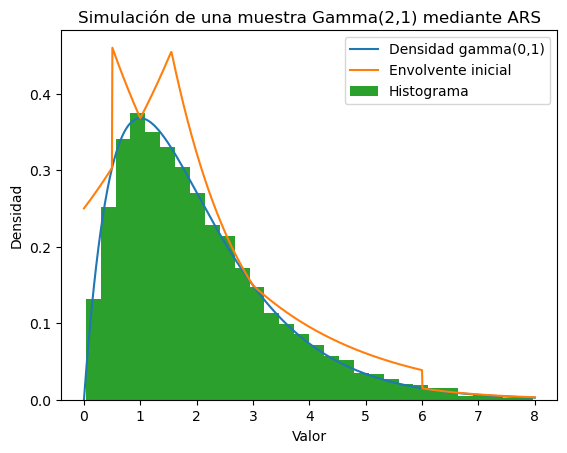
\includegraphics[width=0.6\textwidth]{hist_gamma_env.png}
    \end{center}

    Por lo menos visualmente, el ajuste del histograma a la densidad parece ser adecuado. Podemos
    obtener la media y varianza de los datos muestrados para compararlos con los de la distribución
    objetivo. La media y varianza muestrales son, respectivamente, 2.0203555 y 1.9114250, mientras que
    las teóricas son 2 y 2. La prueba de Kolmogorov-Smirnov para la muestra simulada y una gamma(2,1)
    nos arroja un p-valor de 0.1313849, por lo que no hay evidencia estadística suficiente para 
    rechazar la hipótesis nula de que la muestra proviene de una distribución gamma(2,1).

   
\end{enumerate}




 \end{document}